% !TEX root = MAIN.tex


\subsection{Test Suite Evaluation Based on Code-driven Mutation}
\label{sec:codeDriven}

The following requirements regard the Test Suite Evaluation Based on Code-Mutation functionality of the \FAQAS.

\begin{figure}
	\centering
		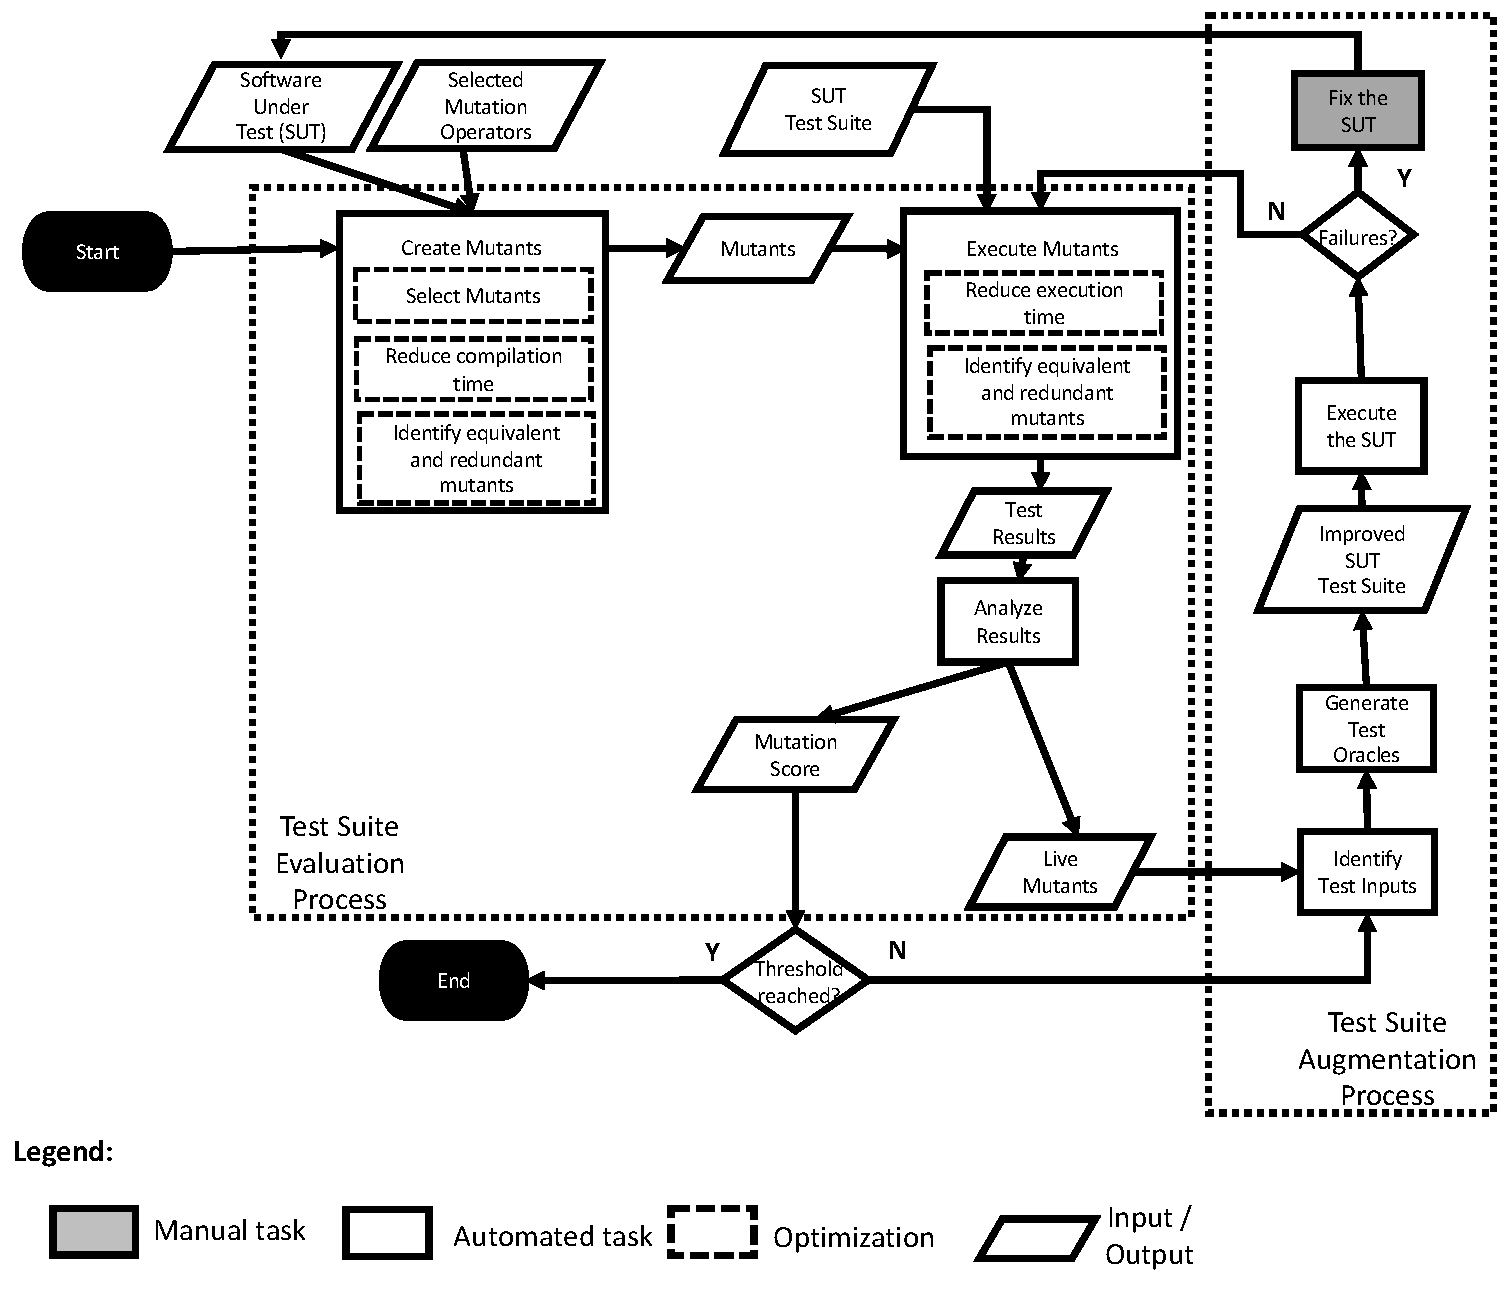
\includegraphics[width=\textwidth]{images/process}
		\caption{Mutation Testing Process.}
		\label{fig:code:process}
	\end{figure}


\RQ{} The \FAQAS shall implement a set of optimizations to make code-driven mutation testing feasible (see D2).

\RQ{} The \FAQAS shall implement the following optimization steps:
\begin{enumerate}
	\item Generate mutants based on code coverage;
	\item Generate mutants based on the sufficient set of operators;
	\item Discard equivalent and redundant mutants based on trivial compiler optimizations;
	\item Sample mutants based on proportional uniform sampling, proportional method-based sampling, uniform fixed-size sampling, and uniform FSCI sampling;
	\item Execute test suites prioritized and reduced based on code coverage;
	\item Discard equivalent mutants based on code coverage.
\end{enumerate}

\RQ{} The \FAQAS shall provide means to enable engineers to run code-driven mutation testing on the SUT.

\RQ{} The \FAQAS shall provide means to enable engineers to select the optimization steps to be carried on the SUT.
%\DONE{I think first we should indicate what are the optimizations supported by FAQAS}

\RQ{} The \FAQAS shall receive as input code coverage information of the SUT.

\RQ{} The \FAQAS shall support test case execution following the practice for the SUT (e.g., running the command \texttt{make test}).

\RQ{} The \FAQAS shall mutate the source code of the SUT.

\RQ{} The \FAQAS shall support C-coded software.

\RQ{} The \FAQAS shall mutate the SUT by applying a set of mutation operators that can be selected by the engineer.

\RQ{} The \FAQAS shall implement the set of operators listed in Table~\ref{table:operators}.

% !TEX root =  ../Main.tex

\newcommand{\op}{\mathit{op}}
\newcommand{\ArithmeticSet}{ \texttt{+}, \texttt{-}, \texttt{*}, \texttt{/}, \texttt{\%} }
\newcommand{\LogicalSet}{ \texttt{&&}, \texttt{||} }
\newcommand{\RelationalSet}{ \texttt{>}, \texttt{>=}, \texttt{<}, \texttt{<=}, \texttt{==}, \texttt{!=} }
\newcommand{\BitWiseSet}{ \texttt{\&}, \texttt{|}, \land }
\newcommand{\ShiftSet}{ \texttt{>>}, \texttt{<<} }


\begin{table}[h]
\caption{Implemented set of mutation operators.}
\label{table:operators} 
\centering
\scriptsize
\begin{tabular}{|@{}p{4mm}@{}|@{}p{2cm}@{\hspace{1pt}}|@{}p{11.1cm}@{}|}
\hline
&\textbf{Operator} & \textbf{Description$^{*}$} \\
\hline
\multirow{7}{*}{\rotatebox{90}{\emph{Sufficient Set}}}&ABS               & $\{(v, -v)\}$	\\
\cline{2-3}
&AOR               & $\{(\op_1, op_2) \,|\, \op_1, \op_2 \in \{ \ArithmeticSet \} \land \op_1 \neq \op_2 \} $       \\
&    			  & $\{(\op_1, \op_2) \,|\, \op_1, \op_2 \in \{\texttt{+=}, \texttt{-=}, \texttt{*=}, \texttt{/=}, \texttt{\%} \texttt{=}\} \land \op_1 \neq \op_2 \} $       \\
\cline{2-3}
&ICR               & $\{i, x) \,|\, x \in \{1, -1, 0, i + 1, i - 1, -i\}\}$           \\
\cline{2-3}
&LCR               & $\{(\op_1, \op_2) \,|\, \op_1, \op_2 \in \{ \texttt{\&\&}, || \} \land \op_1 \neq \op_2 \}$            \\
&				  & $\{(\op_1, \op_2) \,|\, \op_1, \op_2 \in \{ \texttt{\&=}, \texttt{|=}, \texttt{\&=}\} \land \op_1 \neq \op_2 \}$            \\
&				  & $\{(\op_1, \op_2) \,|\, \op_1, \op_2 \in \{ \texttt{\&}, \texttt{|}, \texttt{\&\&}\} \land \op_1 \neq \op_2 \}$            \\
\cline{2-3}
&ROR               & $\{(\op_1, \op_2) \,|\, \op_1, \op_2 \in \{ \RelationalSet \}\}$            \\
&				  & $\{ (e, !(e)) \,|\, e \in \{\texttt{if(e)}, \texttt{while(e)}\} \}$ \\
\cline{2-3}
&SDL               & $\{(s, \texttt{remove}(s))\}$            \\
\cline{2-3}
&UOI               & $\{ (v, \texttt{--}v), (v, v\texttt{--}), (v, \texttt{++}v), (v, v\texttt{++}) \}$            \\   
\hline
\hline
\multirow{5}{*}{\rotatebox{90}{\emph{OODL}}}&AOD               & $\{((t_1\,op\,t_2), t_1), ((t_1\,op\,t_2), t_2) \,|\, op \in \{ \ArithmeticSet \} $       \\ 
\cline{2-3}
&LOD               & $\{((t_1\,op\,t_2), t_1), ((t_1\,op\,t_2), t_2) \,|\, op \in \{  \} \}$       \\ 
\cline{2-3}
&ROD               & $\{((t_1\,op\,t_2), t_1), ((t_1\,op\,t_2), t_2) \,|\, op \in \{ \RelationalSet \} \}$       \\ 
\cline{2-3}
&BOD               & $\{((t_1\,op\,t_2), t_1), ((t_1\,op\,t_2), t_2) \,|\, op \in \{ \BitWiseSet \} \}$       \\ 
\cline{2-3}
&SOD               & $\{((t_1\,op\,t_2), t_1), ((t_1\,op\,t_2), t_2) \,|\, op \in \{ \ShiftSet \} \}$       \\ 
%\hline
%COR               & $\{(\op_1, \op_2) \,|\, \op_1, \op_2 \in \{ \texttt{\&\&}, \texttt{||}, \land \} \land \op_1 \neq \op_2 \}$            \\
\hline
\hline
\multirow{3}{*}{\rotatebox{90}{\emph{Other}}}&LVR			& $\{(l_1, l_2) \,|\, (l_1, l_2) \in \{(0,-1), (l_1,-l_1), (l_1, 0), (\mathit{true}, \mathit{false}), (\mathit{false}, \mathit{true})\}\}$\\
&&\\
&&\\
\hline
\end{tabular}

$^{*}$Each pair in parenthesis shows how a program element is modified by the mutation operator. Th eleft element of the pair is replaced with the right element. We follow standard syntax~\cite{kintis2018effective}. Program elements are literals ($l$), integer literals ($i$), boolean expressions ($e$), operators ($\op$), statements ($s$), variables ($v$), and terms ( $t_i$, which might be either variables or literals).
\end{table}

\RQ{} The \FAQAS shall apply all available mutation operators in case they are not specified.

\RQ{} The \FAQAS shall store every generated mutant on a directory tree that follows the structure of the source directory tree of the SUT.

\remark Every source file is replaced by a folder; the folder has the same name of the file. The folder contains all the mutants generated for that file.

\RQ{} The \FAQAS shall generate mutants with unique name identifiers.

\RQ{} The \FAQAS shall generate mutants with names that results from the conjunction of the following information:
source file name, mutated function name, mutated line, mutation operator name, mutation operation, mutated ``column'' (i.e., char position from the beginning of the line).

\RQ{} The \FAQAS shall compile mutants incrementally to save compilation time.

\RQ{} The \FAQAS shall disregard equivalent and redundant mutants based on trivial compiler equivalence.

% not sure if we should keep this
\RQ{} The \FAQAS shall work with compilation scripts that are modified by the engineer according to rules specific for the \FAQAS.
%Fabrizio: the subject should always be FAQAS
%The engineer shall provide a modified compilation script for the SUT (e.g., the \emph{Makefile}).
The modified compilation script (i) shall not contain debugging nor coverage flags, (ii) shall contain a placeholder for the compiler optimization option, and (iii) shall contain a 'sort' command in the source dependency list to ensure that source files are always compiled in the same order.

\RQ{} The \FAQAS shall compile every mutant with the \textit{O0}, \textit{O1}, \textit{O2}, \textit{O3}, \textit{Ofast}, and \textit{Os} GCC compiler optimisation options\footnote{https://gcc.gnu.org/onlinedocs/gcc/Optimize-Options.html}.

\RQ{} The \FAQAS shall generate a SHA512 hash for every compiled mutant to enable mutant comparisons.

\RQ{} The \FAQAS shall disregard mutants that generate a compilation error.

\RQ{} The \FAQAS shall not disregard mutants that produce a compilation warning.

\RQ{} The \FAQAS shall a produce a list of nonequivalent and nonredundant mutants based on trivial compiler equivalence.

%Fabrizio: it was fitting the implementation, not the problem to address
\RQ{} The \FAQAS shall generate a set of prioritized and reduced test suites for every mutant.
%covered statement within the SUT.
The generation of such test suites should be  based on the PrioritizeAndReduce Algorithm (See D2).

\RQ{} The \FAQAS shall provide an option to execute only the prioritized and reduced set of test cases when testing a mutant affecting a certain statement. When the option is disabled, the \FAQAS shall execute the whole test suite for every mutant. The execution of a test suite shall be stopped when a mutant is killed.

\RQ{} The \FAQAS shall support strong mutation testing (see D2).

\RQ{} The \FAQAS shall sample the mutants to be executed.

\RQ{} The \FAQAS shall support the mutant selection strategy \textit{all mutants} (see D2).

\RQ{} The \FAQAS shall support the mutant selection strategy \textit{proportional uniform sampling} (see D2).

\RQ{} The \FAQAS shall support the mutant selection strategy \textit{proportional method-based sampling} (see D2).

\RQ{} The \FAQAS shall enable engineers to provide a sampling rate if \textit{proportional uniform sampling} or \textit{proportional method-based sampling} is selected.

\RQ{} The \FAQAS shall support the mutant selection strategy \textit{uniform FSCI sampling} (see D2).

\RQ{} The \FAQAS shall compile a mutant by running the build script of the original program.

\RQ{} The \FAQAS shall support simple runtime optimizations:
\begin{enumerate}
	\item stopping the execution of the test suite when the mutant has been killed,
	\item executing only those test cases that cover the mutated statements, and
	\item rely on timeouts to automatically detect infinite loops introduced by mutation.
\end{enumerate}

%\RQ{} The \FAQAS shall execute the SUT test suite for every mutant.

\RQ{} The \FAQAS shall compile and execute mutants till a termination criterion is met. The termination criterion depends on the mutants selection strategy (see D2 for details):
\begin{itemize}
	\item \emph{all mutants}: all mutants have been executed
	\item \emph{proportional uniform sampling}: a number of mutants matching the selected percentage has been executed
	\item \emph{proportional method-based sampling}: a number of mutants matching the selected percentage for all methods in the SUT has been executed
	\item \emph{uniform fixed-size sampling}: a number of mutants matching the selected value has been executed
	\item \emph{uniform FSCI sampling}: the confidence interval computed is smaller than 10\%.
\end{itemize}


\RQ{} The \FAQAS shall identify equivalent mutants based on code coverage information using the distance criterion $D_C$ (see D2).

%\RQ{} The \FAQAS shall disregard all the equivalent mutants from the mutation results.

\RQ{} The \FAQAS shall compute the mutation score of the SUT based on mutation results. Equivalent mutants shall not be considered for the computation of the mutation score (see D2).

\RQ{} The \FAQAS shall produce two prioritized lists (list A and list B) of live and nonequivalent mutants.
%\TODO{We have to discuss the meaning of the following sentence}
List A should contain live mutants that shall be inspected first by the engineers because different from the SUT (i.e., nonequivalent) and different from each other. Ideally, each mutant in list A should represent a distinct limitation of the SUT.
List A contains mutants that have a distance $D_C$ (strictly) greater than zero; in other words, the distance between each pair of mutants appearing in list A should be greater than zero.
List B contains all the remaining live, nonequivalent mutants.
The two lists are sorted in decreasing order, based on the distance $D_C$ from the original program.

\remark Equivalent mutants, which are discarded, have a distance $D_C$ from the original program equal to zero.
The generation of the list proceeds as follows. First, a list (list X) containing all the mutants, sorted by distance $D_C$, is created. Iteratively, each mutant in list X is compared with each mutant in list A. If the distance is greater than zero, the mutant is added to list A, otherwise it is added to list B.


\RQ{} The \FAQAS shall report a summary of the results obtained in every step of the mutation testing process.

% test suite augmentation


\subsection{Test Suite Augmentation Based on Code-driven Mutation}
\label{sec:codeDrivenAugmentation}

The following requirements regard the Test Suite Augmentation functionality aiming to generate test cases that kill mutants generated with the Code-driven Mutation functionality of the \FAQAS.

\RQ{} The \FAQAS shall support test suite augmentation based on code mutation.

\RQ{} The \FAQAS shall rely on the KLEE test case generation tool to support test suite augmentation.

\RQ{} For each live mutant, the \FAQAS should generate test scaffoldings that are processed by KLEE.

\RQ{} The \FAQAS shall provide the engineer with the ability to configure the generated test scaffoldings.


\remark For example, the \FAQAS shall provide the engineer with the ability to refine the generated assertions. Since assertions concern output and state variables, it is necessary to verify that all the necessary output/state variables had been referred in assertion. Indeed, in C, with pointers and pointers to pointers, it is not possible to have a precise automated identification of output/state variables.

\RQ{} The \FAQAS shall generate a tentative unit test case (i.e., a source file in C) that kills the mutants.

\remark  The \FAQAS may generate test cases consisting of (i) an invocation of the function under test (i.e., the function targeted by the mutation), (ii) its assigned arguments, and (iii) an assertion that verifies results.

%\RQ{} The engineer shall inspect the generated test cases by verifying that KLEE has generated valid inputs (e.g., inputs that meet the program preconditions).
%
%\RQ{} The engineer shall inspect the generated test cases by verifying that the generated assertion with the expected value is correct (i.e., it reflects what indicated in the SUT specifications).
%
%\remark If the value appearing in the assertion is not correct, it means that KLEE during its execution has observed an incorrect value being generated by the SUT; for this reason, the SUT might be faulty and should be fixed.
%
%\RQ{} The engineer shall add manually the generated test case to the test suite.
%
%\RQ{} The engineer shall inspect manually the mutant for equivalence when a test case is not generated.
%
%\RQ{} The engineer shall remove the mutant from the mutation results, if the manual inspection of mutant equivalence is positive.
%
%\RQ{} The \FAQAS shall recompute the mutation score after ignoring the equivalent mutants detected by KLEE.
